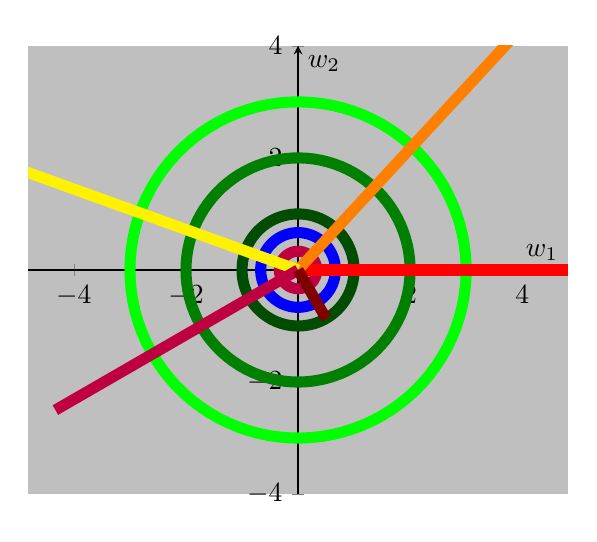
\begin{tikzpicture}
	\begin{axis}[
		axis lines=middle,
		axis equal,
		xmin=-4,
		xmax=4,
		ymin=-4,
		ymax=4,
		xlabel=$w_1$,
		ylabel=$w_2$,
		axis background/.style={fill=gray!50}
	]	
		\addplot [domain=-180:180, samples=100, color=green, line width=4pt] ({3*cos(x)}, {3*sin(x)});
		\addplot [domain=-180:180, samples=100, color=black!50!green, line width=4pt] ({2*cos(x)}, {2*sin(x)});
		\addplot [domain=-180:180, samples=100, color=black!70!green, line width=4pt] ({cos(x)}, {sin(x)});
		\addplot [domain=-180:180, samples=100, color=blue, line width=4pt] ({2/3*cos(x)}, {2/3*sin(x)});
		\addplot [domain=-180:180, samples=100, color=purple, line width=4pt] ({1/3*cos(x)}, {1/3*sin(x)});
		
		\addplot[-, red, line width=4pt] coordinates {(0, 0) (5, 0)};
		\addplot[-, orange, line width=4pt] coordinates {(0, 0) ({8*cos(60)}, {5*sin(60)})};
		\addplot[-, yellow, line width=4pt] coordinates {(0, 0) ({8*cos(150)}, {5*sin(150)})};
		\addplot[-, purple, line width=4pt] coordinates {(0, 0) ({5*cos(-150)}, {5*sin(-150)})};
		\addplot[-, black!50!red, line width=4pt] coordinates {(0, 0) ({cos(-60)}, {sin(-60)})};
	\end{axis}
\end{tikzpicture}